\section{Introduction}
\label{sec:intro}
\begin{figure}[h]
\centering
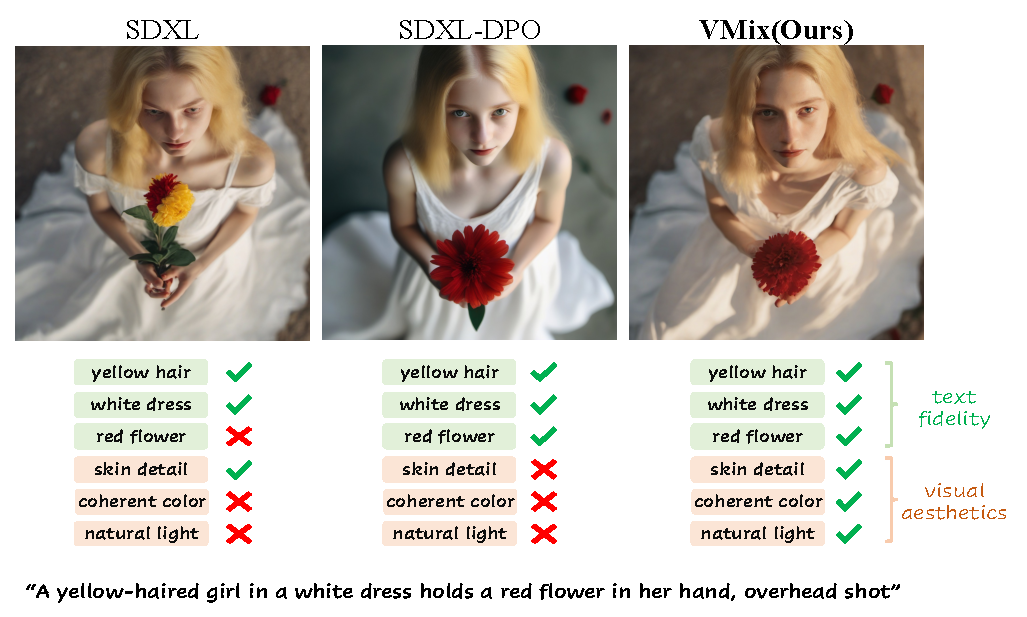
\includegraphics[scale=0.48]{aes_dpo_vmix_compare.pdf}
    \caption{Comparison of text fidelity and visual aesthetics between SDXL~\cite{podell2023sdxl}, DPO~\cite{wallace2024diffusion}, and our VMix. DPO can generate attributes that SDXL fails to produce, but it fails to align with human visual fine-grained preferences. Our method achieves better text fidelity and visual aesthetics simultaneously.}
    \label{Figure 0}
\end{figure}
The past few years have witnessed the flourish in the field of text-to-image generation, especially the advent of large-scale pretrained text-to-image diffusion models\cite{rombach2022high,nichol2021glide,ramesh2022hierarchical,feng2023ernie,podell2023sdxl}, allowing human to create visually compelling images using text prompts conveniently.
Although these large models can produce overall high-quality images in visual realism and textual alignment, the current results still exhibit significant gaps from human expectations in various aspects, such as generated images with unnatural lighting, distorted human bodies, or supersaturated colors.
These misalignment with human expectation is fatal for the real-world applications of AI-generated content such as film production, since human beings are highly sensitive to these \emph{``devils in the details"}.
Therefore, the key challenge has become how to accurately align the generated images with human preference across various aspects.

Existing works have made considerable efforts to improve image quality to meet human preferences, which can be primarily categorized into two streams.
The first stream focuses on fine-tuning the pre-trained text-to-image models either based on an exceptionally high-quality sub-dataset\cite{dai2023emu}, or based on reward models via reinforcement learning\cite{liang2024rich, xu2024imagereward, kirstain2023pick} and direct preference optimization(DPO)\cite{wallace2024diffusion}.
The latter stream\cite{si2023freeu, he2024freestyle} instead focuses on investigating the generation behavior of pre-trained diffusion models itself to improve its generation stability.
For example, FreeU\cite{si2023freeu} proposed re-weighting the contributions sourced from skip connections and backbones in the denoising model to strengthen the denoising ability while simultaneously enhancing details.
In summary, existing methods align the generation results with human preference by improving the overall generation quality in terms of visual realism or textual consistency.

However, in this study, we argue that existing methods fail to align \emph{fine-grained human preference} for visually generated content.
Images favored by human beings should excel across various fine-grained aesthetic dimensions simultaneously, such as natural light, coherent color, and reasonable composition.
On the one hand, these fine-grained aesthetic demands can not be simply addressed by augmenting detailed textual descriptions for pretrained diffusion models to understand.
The reason is that their text encoders (\emph{e.g.}, CLIP\cite{radford2021learning} or T5\cite{raffel2020exploring}) are primarily trained for capturing high-level semantics and lacking the accurate awareness for these ineffable visual aesthetics.
On the other hand, the optimization direction for overall image generation quality is neither equivalent to nor consistent with the direction for these fine-grained aesthetic dimensions. 
For instance, while overall better-generated results may exhibit greater textual alignment, they might suffer from poorer visual composition, as depicted in \cref{Figure 0}.

To address this challenge, we introduce \textbf{VMix}, a novel plug-and-play adapter designed to systematically bridge the aesthetic quality gap between generated images and real-world counterparts across various aesthetic dimensions. 
We finetune the adapter on a hand-selected subset of exceptionally high-quality images derived from a large corpus. Inspired by universal photography standards, which encompass aspects like color, lighting, composition, and focus~\cite{dai2023emu}, we label these images across various aesthetic dimensions.
During training, we freeze the base model and employ the LoRA\cite{hu2021lora} method to ensure practical applicability.
We further design two specialized modules to incorporate these aesthetic labels as additional conditions into the U-Net~\cite{ronneberger2015u} architecture. The first, termed the \emph{aesthetic embedding initialization module}, pre-processes the aesthetic textual data, initializing it into embeddings that align with the corresponding images. 
This step is essential only at the commencement of training. 
Once training begins, we map the aesthetic labels of various images to embeddings by referencing the initial results. 
To better integrate this embedding into the U-Net, we introduce the second module, the \emph{cross-attention mixing control module}, which aims to minimize adverse effects on image-text alignment without directly altering the attention maps.
Our extensive experiments demonstrate that VMix can be seamlessly integrated with various base models, significantly enhancing their aesthetic performance. Moreover, VMix exhibits excellent compatibility with community modules (i.e., ControlNet\cite{zhang2023adding}, IP-Adapter\cite{ye2023ip}, and LoRA\cite{hu2021lora}), thereby providing the community with greater creative capabilities.

In summary, our main contributions are:
\begin{itemize}
    \item We analyze and explore the differences in generated images across fine-grained aesthetic dimensions, proposing the disentanglement of these attributes in the text prompt to provide a clear direction for model optimization. 
    \item We introduce VMix, which disentangles the input text prompt into content description and aesthetic description, offering improved guidance to the model via a novel condition control method called value-mixed cross-attention.
    \item The proposed VMix approach is universally effective for existing diffusion models, serving as a plug-and-play aesthetic adapter that is highly compatible with community modules.
\end{itemize}
